\subsection{Credibilidad y calidad de los datos}
Es indispensable  serciorarse en primer lugar de la credibilidad del conjunto de datos, es decir, la fuente debe ser fiable. Normalmente,
en la descripcion de los datos debe contar una seccion dende explique la procedencia del conjunto datos.

Respecto a la calidad del conjunto de datos, se puede medir acorde a las siguientes caracteristicas de los valores de los campos:\\

\textbf{Precision}. Unidades de medida en la escala correcta. Por ejemplo, si estamos mediendo la altura
de las personas, carecera de sentido proporcionar estas medidas en metros, ya que los posibles valores, seran 0, 1 y 2.\\

 \textbf{Consistencia}. Valores logicos para cada tipo de campo. Un ejemplo seria un campo fecha, todos deberian
seguir el mismo formato.\\

\textbf{Interpretabilidad}. Legible. Los datos deber ser claros, tantos en valores como en unidades. Por ejemplo, no podemos
suponer la unidad o la escala de los datos o, si los datos son dictonicos, "verdadero" o "falso", y los valores represetados son 
"A" o "B", no podemos suponer verdadero= A y falso=B sin que esta informacion este descrita. \\

\textbf{Complitud}. Los datos deben ser consistentes en cada uno de las muestras. Las muestras pueden diferenciarse
 unas de otras, como vemos en la Figura  a continuacion, pueden compartir algunos campos y otros no. Para un buen resultado, seria 
conveniente un grado de complitud alto para los datos que nos interesan en nuestro diseno.


\begin{figure}[ht]
\centering
\framebox{
\vbox{\begin{tabbing} 
Document \\
\hspace*{5mm} \= Sample 1 \\
\hspace*{10mm}\textit{Field A:} \hspace*{5mm} \= value A \\
\hspace*{10mm}\textit{Field B:} \hspace*{5mm} \= value B \\
\hspace*{5mm} \= Sample 2 \\
\hspace*{10mm}\textit{Field A:} \hspace*{5mm} \= value A \\
\hspace*{10mm}\textit{Field C:} \hspace*{5mm} \= value C \\
\hspace*{10mm}\textit{Field D:} \hspace*{5mm} \= value D \\
\hspace*{5mm} \= ... 
\hspace*{5mm} \= Sample n \\
\hspace*{10mm} \= ... 
\end{tabbing}}%
}
\caption{Ejemplo documento de la fuente de origen}
\end{figure}
\begin{comment}
    
\end{co}
\begin{itemize}

    \item Informacion precisa
    \item Datos contrastados
\end{itemize}
\end{comment}


\subsubsection{How to solve it} 
El primer paso es contrastar la informacion con la fuente de origen. Con el conjunto de datos y la definicion
de cada uno de los campos, se ha de comprobar la escala e interpretabilidad de los campos y valores.
A continuacion podemos realizar diferentes analisis de los datos para comprobar su consistencia y complitud. Esto 
es posible realizando distintos graficos y ver si existen valores extremos o extranos.
Herramientas de analisis de bases de datos podran decirnos la complitud de los campos, es decir, que porcentaje de las
muestras contienen cada campo.

\subsubsection{How we solve it. Aire Guru} 
La fuente de dato queda verificada tanto por el CEMI (centro de informatica de Malaga) y UrbanClouds, la empresa privada
que recoge y envia los datos al ayuntamiento de Malaga.
Con la descripcion de los datos en el portal de datos abiertos de Malaga y la informacion recibida por UrbanClouds, 
obtenemos toda la informacion necesaria para interpretar el conjunto de datos.\\

Para cada campo, se ha realizado un estudio grafico con la herramienta Tableau y si ha verificado que los valores de los
campos cumplen con la escala y el rango de valores esperados. Es decir, son precisos y consistentes.
Utilizando las herramientas de analisis de MongoDBCompas y NoSQLBooster comprobamos la complitud de los campos que nos
interensan para nuestro modelo.
\begin{figure}[ht]
    \centering
    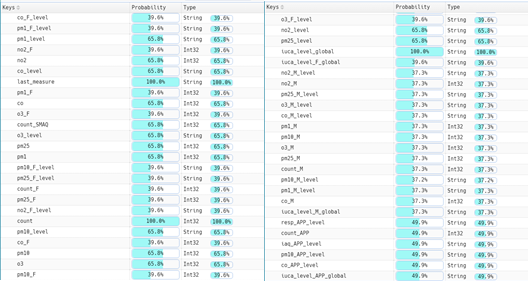
\includegraphics[width=12cm]{noSQLBoosterAnalysis}
    \caption{Analisis de complitud}
\end{figure}

\elsparagraph{Evaluation}  
\begin{itemize}
    \done Se han tomado las medidas necesarias para verificar y entender cada uno de los campos en el conjunto de datos
    \done Se ha analizado los valores de cada uno de los campos comprobando escalas y rangos
    \done Se ha analizado la complitud de los datos
    
\end{itemize}
 \newpage